\documentclass[polish, 11pt]{article}
    
\usepackage[a4paper, margin=25mm]{geometry}
\usepackage{babel,polski}
\usepackage[utf8]{inputenc}
\usepackage[T1]{fontenc}

\usepackage{eso-pic,graphicx}
\newcommand\BackgroundPic{%
\put(0,0){%
\parbox[b][\paperheight]{\paperwidth}{%
\vfill
\centering
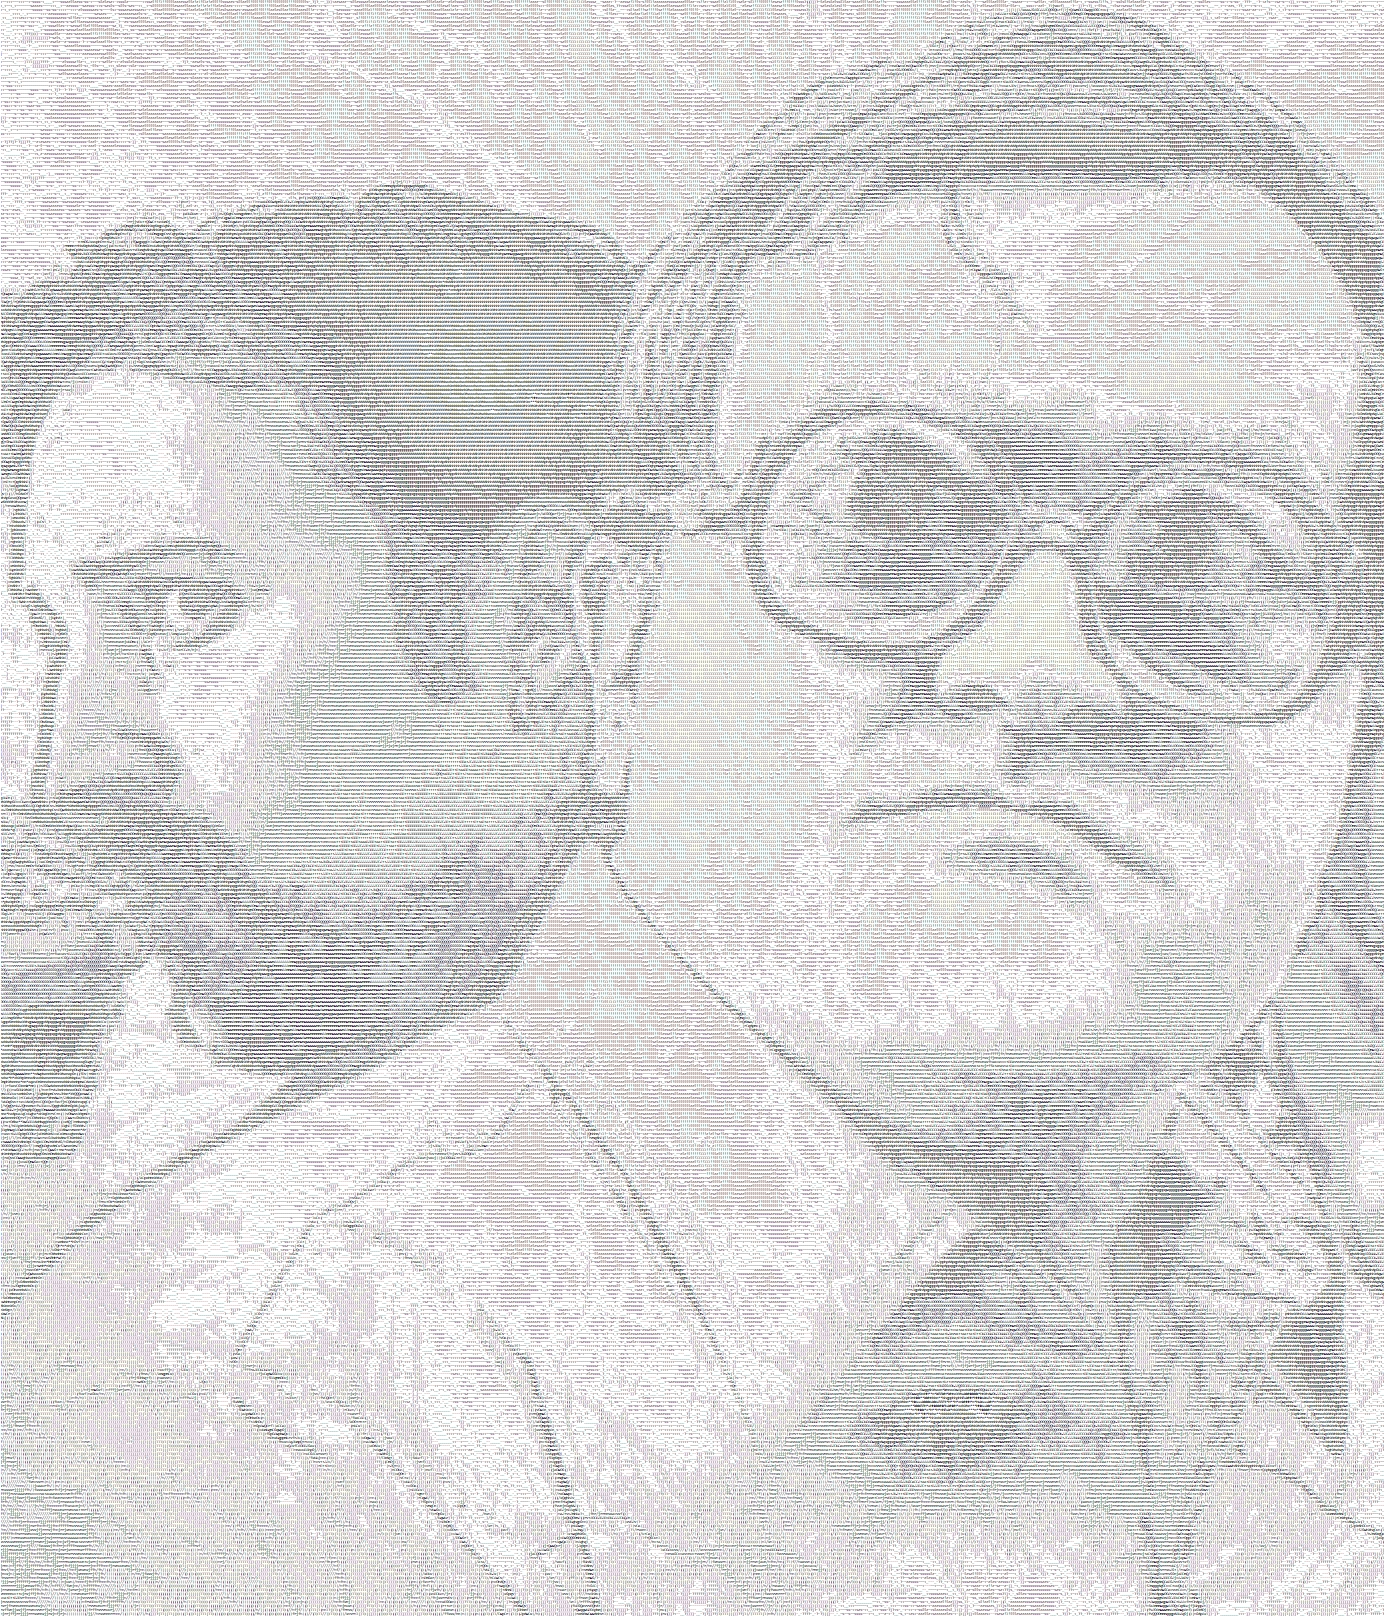
\includegraphics[width=0.9\paperwidth,height=0.9\paperheight]{trailer.jpg}%
\vfill
}}}

\usepackage{pst-text}
\DeclareFixedFont{\RM}{T1}{ptm}{b}{n}{2cm}

\usepackage{lmodern}
\usepackage{xcolor}
\usepackage{listings}
\usepackage{gasasm}
\lstset{language=[GAS]Assembler}

\begin{document}
\begin{titlepage}
    \AddToShipoutPicture*{\BackgroundPic}
    \centering

  \pscharpath[fillstyle=solid,fillcolor=magenta!50]{\RM TeXnik}
    {\scshape\LARGE Architektura komputerów 2\\ projekt \par}
    \vspace{1cm}
    {\scshape\Large,,Konwertowanie plików graficznych w formacie PPM do ciągu znaków ASCII odwzorowującego grafikę''\par}
    \vspace{6cm}
    {\itshape\Large Janusz Długosz --- 235746\/\par}
    {\itshape\Large Marcin Kotas --- 235098\/\par}
    \vfill
    Prowadzący:\par
    Mgr.~Dominik \textsc{Żelazny}

    \vfill

    {\large Wrocław, \today\par}

    %\AddToShipoutPictureBG*{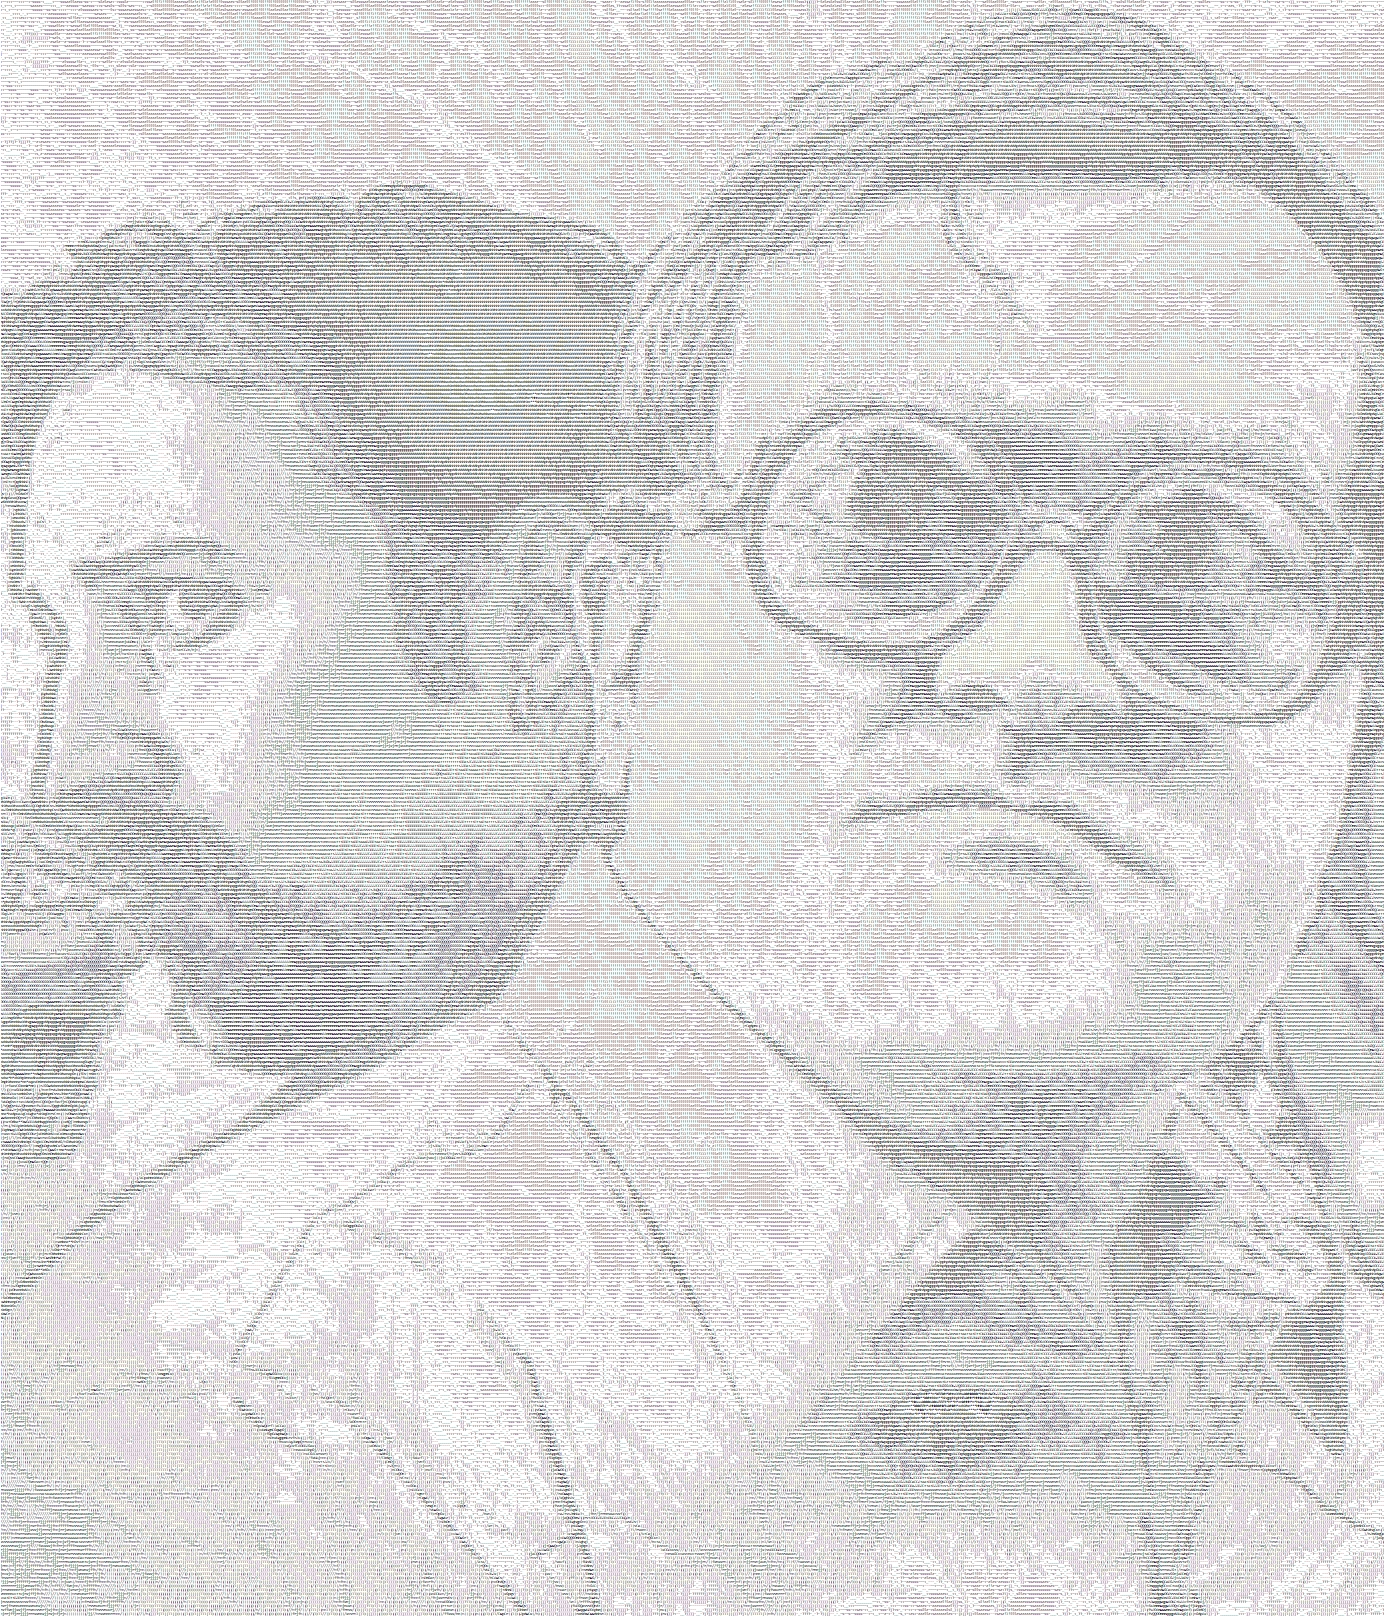
\includegraphics[width=\paperwidth, height=\paperheight]{trailer.jpg}}
    \ClearShipoutPicture

\end{titlepage}

\section{Założenia projektu}
    Plik PPM (ang.\ portable pixmap) – format zapisu grafiki rastrowej,
    w której nie używa się żadnej kompresji.
    Plik zawiera nagłówek z podstawowymi danymi – typ pliku, szerokość, wysokość i maksymalną wartość składową koloru.
    W dalszej części pliku znajdują się wartości składowe kolorów kolejnych pikseli oddzielone spacjami oraz znakami końca linii.
    Przykład:
    \begin{lstlisting}
P3
5 5
255
139 169 195 149 179 205 152 182 208 152 182 208 155 185 211
152 182 208 152 182 208 161 191 217 152 182 208 153 183 209
154 184 210 155 185 211 155 185 211 154 184 210 153 183 209
152 182 208 149 181 206 148 180 205 148 180 205 149 181 206
148 182 207 147 181 206 145 179 204 144 178 203 146 180 205
\end{lstlisting}

    Program będzie wczytywał kolory, a później dzielił obraz na obszary o proporcjach odpowiadającym czcionką o stałej szerokości,
    a następnie obliczał średnią luminancję na danym segmencie i zamieniał ją na odpowiadający jej znak.
    Efekt końcowy powinien odwzorować obraz w stopniu pozwalającym na jego bezproblemową identyfikację.
    Po wykonaniu konwersji ciąg będzie zapisywany do pliku tekstowego.

\section{Etap I}
    W pierwszym etapie stworzona została funkcja wczytująca dane z pliku oraz zapisująca je do trzech oddzielnych buforów (czerwony, zielony, niebieski).
    W osobnych zmiennych zapisywane są informacje definiujące szerokość oraz wysokość obrazu.
    Algorytm pomija linijki rozpoczynające się znakiem oznaczającego komentarz --- `\#'.
    Kolory kolejnych pikseli oddzielone są znakami białymi.
    
    \lstinputlisting[firstline=192,lastline=307]{program/main.s}

\section{Etap II}
    W typ etapie dodana została funkcja obliczająca średnią luminancję pikseli zawierających się w kolejnych prostokątach.
    Prostokąty mają proporcję 1:2 i posiadają zadaną szerokość.
    
    Na początku obraz dzielony jest na prostokąty o wybranym rozmiarze.
    Część, która nadbywa jest ignorowana.
    Funkcja \verb|getRect| przyjmuje jako argument ideks pierwszego piksela danego prostokąta.
    Następnie z tablic \verb|red, green, blue| pobierane są składowe koloru danego piksela.
    Wymnażane są one przez współczynniki według następującego wzoru:
    \begin{displaymath}
        L = \frac{2126\cdot R+7152\cdot G+722\cdot B}{10000}
    \end{displaymath}
    Na koniec funkcja liczy średnią luminancję dla całego prostokąta i zapisuje ją w tablicy \verb|lum|.

    Funkcja wywoływana jest w pętli w głównym programie.
    Pętla ta oblicza indeksy kolejnych prostokątów.

    \lstinputlisting[firstline=97,lastline=133]{program/main.s}
    \lstinputlisting[firstline=341,lastline=388]{program/main.s}

\section{Etap III}
    Na podstawie wyliczonych luminancji dopasowywany jest znak ASCII według następującej skali:\\
    \begin{verbatim}
        "$@B%8&WM*oahkbdpqwmZO0QLCJUYXzvunxrjft/|()1{}]?-_+~<>i!lI:,^`'. "
    \end{verbatim}
    Luminancja w zakresie \verb|0-255| dzielona jest przez 4, aby dopasować do skali 64 stopniowej.
    Następnie znak dobrany ze skali kopiowany jest do bufora wyjściowego \verb|file_out|.

    Bufor \verb|file_out| zapisywany jest do pliku wyjściowego \verb|out.txt|.
    
    \lstinputlisting[firstline=140,lastline=177]{program/main.s}

\section{Wyniki działania programu}

\end{document}